% chapters/chapter2/sec1.tex

\topichead{Purpose of This Chapter}
\label{sec:ch2-prerequisites-purpose}
 

This chapter reviews the digital communication and radar sensing concepts
needed for later discussions of ISAC system models and joint design methods.
It is not intended to replace a complete course on communication or radar
theory.
Instead, it focuses on signal propagation, wireless channels, modulation
waveforms, antenna arrays, receiver processing, and sensing performance
metrics, which together provide the common background for understanding how one
wireless signal may support both information transmission and environmental
sensing.
 


 

\section{Core Principles of Digital Communication}
\label{sec:ch2-digital-comm}


\subsection{Digital Communication Link and Signal Models}

\topichead{Basic Link of a Digital Communication System}

A digital communication system delivers information bits by representing them
as a suitable waveform, transmitting the waveform through a wireless channel,
and recovering the intended information at the receiver under bandwidth, power,
noise, fading, and interference constraints.
Thus, the communication link is both a sequence of functional modules and a
signal-processing chain that determines how information is represented,
transmitted, distorted, and recovered.

This link is also a natural starting point for ISAC.
Rather than attaching sensing as an unrelated module, ISAC exploits components
already present in the communication link: the modulation waveform controls
signal energy in time, frequency, and space; the wireless channel contains
propagation and scattering information; the antenna array provides spatial
selectivity; and the received-signal processing chain supports both symbol
recovery and sensing-parameter extraction.

Fig.~\ref{fig:comm_system_block_diagram} shows a simplified digital
communication link.
\begin{figure}[htbp]
    \centering
    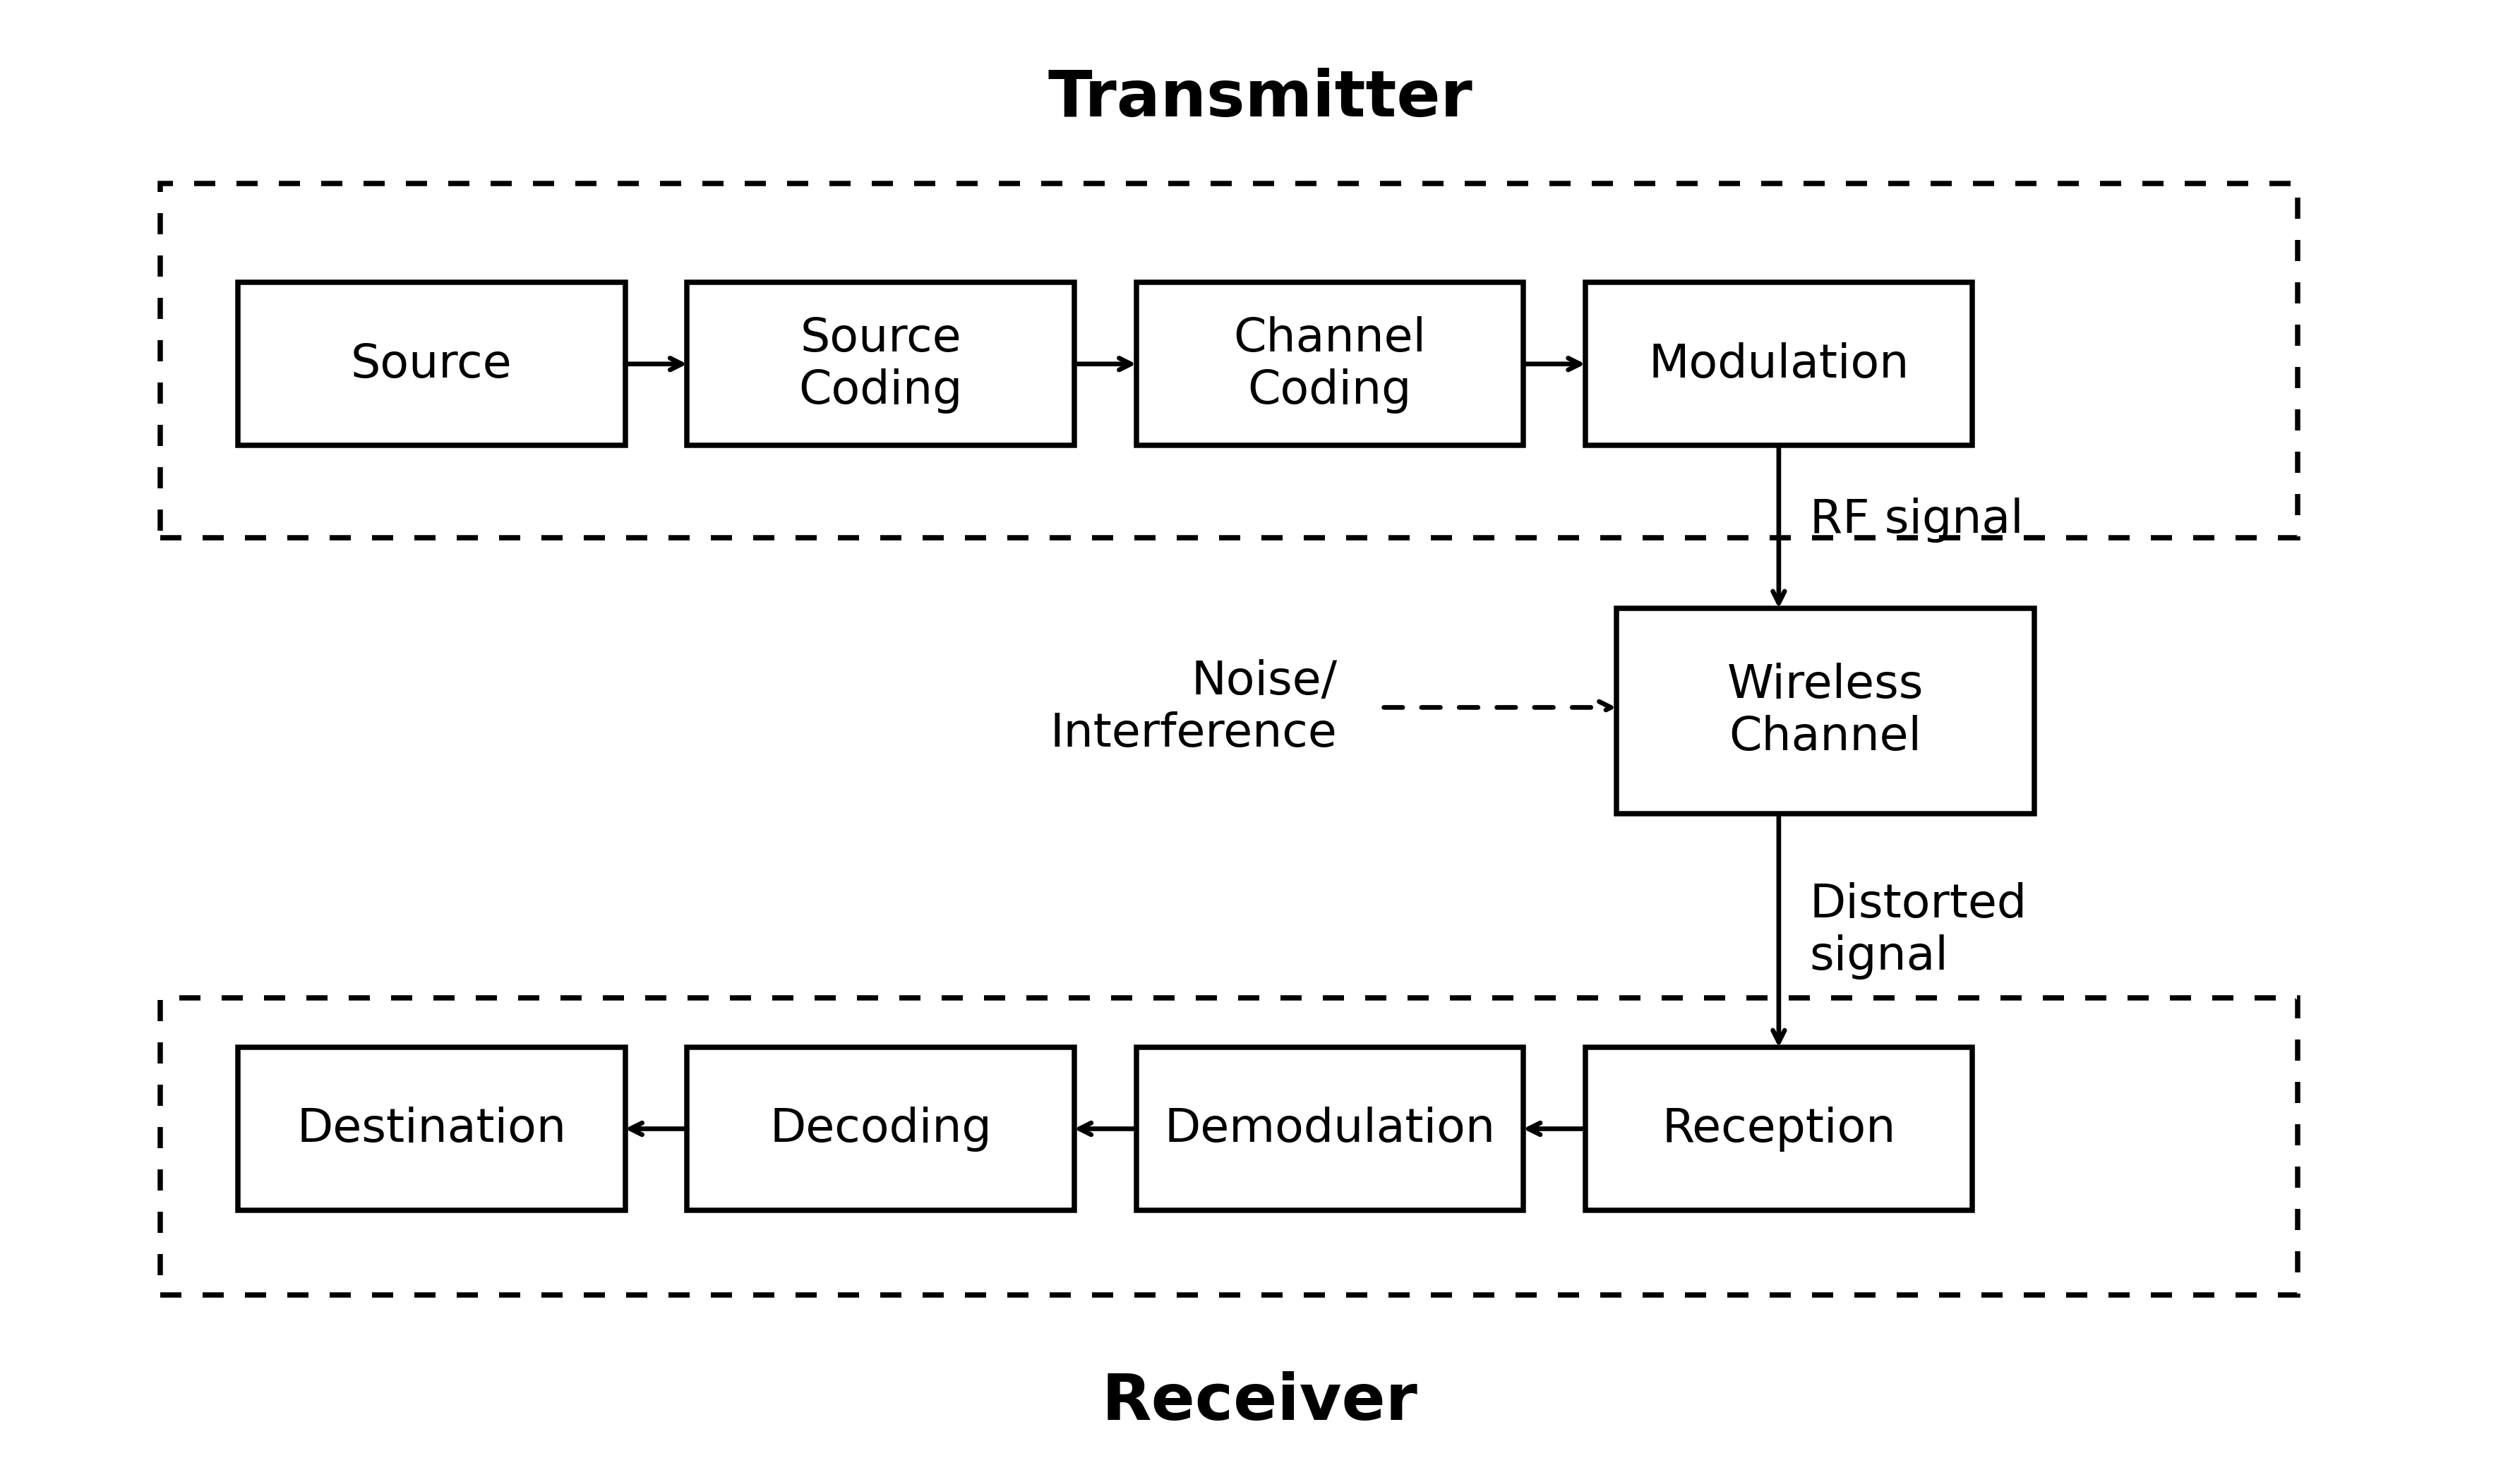
\includegraphics[width=0.72\textwidth]{figures/chapter2/fig_comm_system_block_diagram.png}
    \caption{Basic link diagram of a digital communication system.}
    \label{fig:comm_system_block_diagram}
\end{figure}
\begin{itemize}
    \item \textbf{Information source and source coding:}
    The information source produces raw data such as text, speech, images, or
    sensor measurements, and source coding represents it as a compact bit
    stream.
    These modules determine the communication content, but they are usually not
    the direct source of sensing information in ISAC.

    \item \textbf{Channel coding:}
    Channel coding adds controlled redundancy so that the receiver can detect or
    correct errors caused by noise, fading, and interference.
    In ISAC, it helps maintain communication reliability when time, frequency,
    spatial, or power resources are shared with sensing.

    \item \textbf{Modulation and waveform formation:}
    Modulation maps coded bits to symbols and forms the transmitted waveform.
    Common schemes such as PSK and QAM represent bits through phase or joint
    amplitude-phase changes of the carrier.
    It is one of the most direct bridges to ISAC, because waveform bandwidth,
    duration, subcarrier structure, and correlation properties affect both
    communication efficiency and sensing resolution.

    \item \textbf{Wireless channel:}
    The wireless channel introduces path loss, fading, multipath, noise, and
    interference.
    For communication, these effects are impairments to be estimated or
    compensated; for sensing, the same propagation and reflection effects may
    carry information about range, velocity, angle, and the environment.

    \item \textbf{Antenna array and reception:}
    The receiver captures the propagated signal and performs front-end
    operations such as down-conversion, sampling, and synchronization.
    With multiple antennas, the array response supports beamforming, spatial
    interference management, MIMO communication, and angle-related sensing.

    \item \textbf{Demodulation and decoding:}
    Demodulation estimates the transmitted symbols, while decoding recovers the
    information bits.
    In ISAC, this receiver chain may coexist with echo enhancement, parameter
    estimation, or tracking before the recovered data are delivered to the
    destination.
\end{itemize}
Therefore, the digital communication link identifies the main technical
interfaces through which ISAC integrates waveform design, channel modeling,
MIMO beamforming, receiver processing, and resource allocation.


\topichead{Communication Signal Model}

A basic communication signal model describes the relationship among the
transmitted waveform, the wireless channel, and the received observation in the
presence of noise or interference.
In the time domain, this relationship is commonly represented by
\begin{equation}
    y(t) = h(t) * x(t) + n(t),
    \label{eq:comm_time_domain_model}
\end{equation}
where \(x(t)\) is the transmitted baseband signal,
\(h(t)\) is the impulse response of the wireless channel,
\(n(t)\) is noise or interference,
\(y(t)\) is the received signal,
and \(*\) denotes convolution.
This model shows that the received signal is jointly determined by the
transmitted signal, the channel, and noise.

After the Fourier transform, the convolution becomes a multiplicative
frequency-domain relationship:
\begin{equation}
    Y(f) = H(f)X(f) + N(f).
    \label{eq:comm_frequency_domain_model}
\end{equation}
This form explains how different frequency components are affected by the
channel and provides the basis for OFDM and frequency-domain resource
allocation.

In discrete-time,
multi-carrier,
or multi-antenna systems,
the communication link is also often written in a unified form as
\begin{equation}
    \mathbf{Y} = \mathbf{H}\mathbf{X} + \mathbf{N},
    \label{eq:comm_matrix_model}
\end{equation}
where \(\mathbf{X}\) denotes the transmitted-signal representation after coding
and modulation,
\(\mathbf{H}\) denotes the discrete channel response or channel matrix,
\(\mathbf{N}\) denotes noise or interference,
and \(\mathbf{Y}\) denotes the received-signal representation.
This compact form is widely used in MIMO,
OFDM,
and multi-user communication systems.
It also provides the mathematical starting point for later ISAC models,
where a designed transmit signal interacts with both communication channels
and sensing or target responses before being observed at the receiver.

\topichead{ISAC Signal Model}

The communication signal model above can be extended naturally to ISAC.
In a traditional communication system, the transmitted signal mainly carries
information bits to be demodulated and decoded after propagation.
In an ISAC system, the same signal also illuminates targets or the environment
and carries physical information through reflection, scattering, and related
propagation processes.
Thus, the ISAC signal model needs to describe both communication reception and
sensing echoes.

To reflect this dual function, the received signal can be described through a
communication observation and a sensing observation.
For communication, the received signal keeps a form similar to that of a
traditional link:
\begin{equation}
    \mathbf{Y}_{\mathrm{C}}
    =
    \mathbf{H}\mathbf{X}
    +
    \mathbf{N}_{\mathrm{C}},
    \label{eq:isac_communication_model}
\end{equation}
where \(\mathbf{X}\) denotes the ISAC transmitted signal,
\(\mathbf{H}\) denotes the communication channel matrix,
\(\mathbf{N}_{\mathrm{C}}\) denotes noise or interference at the communication receiver,
and \(\mathbf{Y}_{\mathrm{C}}\) denotes the communication received signal.
The receiver then recovers the information bits carried by \(\mathbf{X}\) from
\(\mathbf{Y}_{\mathrm{C}}\).

For sensing, the same transmitted signal \(\mathbf{X}\) illuminates the target
or environment and generates an echo:
\begin{equation}
    \mathbf{Y}_{\mathrm{R}}
    =
    \mathbf{G}\mathbf{X}
    +
    \mathbf{N}_{\mathrm{R}},
    \label{eq:isac_sensing_model}
\end{equation}
where \(\mathbf{Y}_{\mathrm{R}}\) denotes the echo signal obtained by the sensing receiver,
\(\mathbf{G}\) denotes the target response matrix,
also referred to as the sensing channel in this context,
and \(\mathbf{N}_{\mathrm{R}}\) denotes the noise at the sensing receiver.
Compared with the communication channel \(\mathbf{H}\),
the sensing response \(\mathbf{G}\) has a more explicit physical interpretation:
it is associated with target range,
velocity,
angle,
reflection coefficient,
and scattering characteristics.
The sensing receiver therefore estimates target or environmental parameters
from \(\mathbf{Y}_{\mathrm{R}}\) rather than recovering information bits.

The key difference is therefore not merely the addition of a sensing receiver,
but the dual role of \(\mathbf{X}\): it is both the carrier of information bits
and the illumination signal for probing targets and the environment.
The ISAC model extends the same input--channel--output view, with the important
difference that the channel or response now carries both communication and
sensing meanings.
This view will be used later for waveform design, MIMO beamforming,
communication--sensing tradeoffs, and resource optimization.


\subsection{Wireless Channels and Communication Quality}

\topichead{Basic Concepts of Wireless Channels and Communication Quality}

The signal models introduced above show that both communication reception and
sensing observation are shaped by the transmitted signal,
the propagation environment,
and noise or interference.
For communication,
the wireless channel determines how reliably information symbols can be
recovered at the receiver.
For sensing,
the same propagation process may contain physical information about targets,
scatterers,
and the surrounding environment.

Therefore,
the wireless channel should not be regarded as an ideal or transparent
transmission pipe.
It is affected by propagation distance,
blockage,
multipath reflection,
user mobility,
noise,
and external interference.
These factors determine communication quality metrics such as BER,
throughput,
and spectral efficiency.
In ISAC systems,
they also influence whether useful sensing information can be extracted from
the received signal.

For this reason,
the following discussion reviews several basic concepts:
path loss,
multipath propagation,
fading,
communication quality metrics,
and channel state information.
These concepts provide the necessary background for understanding OFDM,
MIMO beamforming,
and later ISAC joint design.
 
\topichead{Path Loss}

When a wireless signal propagates in space, the received power usually
decreases with distance.
This average attenuation is called path loss, and it describes the most basic
large-scale trend of a wireless channel.

Under ideal free-space propagation conditions,
the received power is commonly described by the Friis transmission formula:
\begin{equation}
    P_r
    =
    P_t G_t G_r
    \left(
        \frac{\lambda}{4\pi d}
    \right)^2 .
    \label{eq:friis-transmission}
\end{equation}
Here, \(P_t\) and \(P_r\) denote the transmit and received powers,
\(G_t\) and \(G_r\) denote the antenna gains, \(\lambda\) is the wavelength,
and \(d\) is the propagation distance.
Eq.~\eqref{eq:friis-transmission} shows that received power depends on
transmit power, antenna gains, distance, and wavelength.
The free-space attenuation is mainly determined by
\[
    \left(
        \frac{\lambda}{4\pi d}
    \right)^2
\]
If the power loss caused by the propagation process itself is represented separately,
the free-space path loss can be written as
\begin{equation}
    \mathrm{FSPL}(d)
    =
    \left(
        \frac{4\pi d}{\lambda}
    \right)^2 .
    \label{eq:free-space-path-loss-linear}
\end{equation}
In engineering analysis,
path loss is usually expressed in dB form as
\begin{equation}
    \mathrm{FSPL}_{\mathrm{dB}}(d)
    =
    20\log_{10}
    \left(
        \frac{4\pi d}{\lambda}
    \right).
    \label{eq:free-space-path-loss-db}
\end{equation}
Accordingly,
the received power in a link budget can also be written as
\begin{equation}
    P_r(\mathrm{dBm})
    =
    P_t(\mathrm{dBm})
    +
    G_t(\mathrm{dB})
    +
    G_r(\mathrm{dB})
    -
    \mathrm{FSPL}_{\mathrm{dB}}(d).
    \label{eq:link-budget-fspl}
\end{equation}
Eq.~\eqref{eq:link-budget-fspl} shows the link-budget role of path loss:
transmit power and antenna gains increase received power, whereas propagation
loss reduces it.

The free-space model is idealized because it assumes a clear line-of-sight
path and ignores blockage, reflection, scattering, and diffraction.
In urban, indoor, industrial, or vehicular scenarios, these factors also affect
received signal strength.
Thus, path loss mainly describes the average distance-dependent trend, while
local fluctuations are better explained by multipath propagation and fading.

\topichead{Multipath Propagation}

In a practical wireless environment, the transmitted signal may reach the
receiver through direct, reflected, scattered, or diffracted paths.
The same transmitted signal is therefore observed as multiple components with
different delays, amplitudes, phases, and angles of arrival; this phenomenon is
called multipath propagation.

In a relatively simple time-invariant multipath channel,
the channel impulse response can be written as
\begin{equation}
    h(\tau)
    =
    \sum_{\ell=1}^{L}
    \alpha_{\ell}
    \delta
    \left(
        \tau-\tau_{\ell}
    \right),
    \label{eq:time-invariant-multipath-channel}
\end{equation}
where \(L\) is the number of resolvable paths, \(\alpha_{\ell}\) is the
complex gain of the \(\ell\)-th path, \(\tau_{\ell}\) is its delay, and
\(\delta(\cdot)\) is the impulse function.
The received signal can thus be viewed as a superposition of delayed copies.

When the transmitter, receiver, or scatterers move, the multipath channel
becomes time-varying and can be written as
\begin{equation}
    h(t,\tau)
    =
    \sum_{\ell=1}^{L}
    \alpha_{\ell}(t)
    \delta
    \left(
        \tau-\tau_{\ell}(t)
    \right),
    \label{eq:time-varying-multipath-channel}
\end{equation}
where \(\alpha_{\ell}(t)\) and \(\tau_{\ell}(t)\) denote the time-varying
complex gain and delay.
With mobility, each path may also contain Doppler and angle information, so a
multipath channel may vary in delay, time, frequency, and space.

For communication, multipath changes the amplitude, phase, and delay structure
of the received signal and may cause distortion, ISI, or received-power
fluctuations.
In MIMO systems, however, rich scattering can also provide spatial degrees of
freedom for diversity gain and spatial multiplexing.
For ISAC, multipath has a more direct physical meaning: different paths may
correspond to targets, reflectors, or scattering structures and may carry range,
velocity, angle, and reflection information.
When these components overlap and vary in time, frequency, or space, the
received signal further exhibits fading.


\topichead{Fading}

Fading refers to variations in the amplitude, phase, or power of the received
signal over space, time, or frequency.
It results from propagation distance, blockage, multipath, mobility, carrier
frequency, and the surrounding environment.
Path loss and shadowing affect average received power, multipath superposition
causes local fluctuations, and motion makes the channel time-varying.
Fading is therefore commonly understood from spatial, temporal, and frequency
perspectives.


\noindent\textbullet\quad\textbf{From the spatial scale: large-scale fading and small-scale fading}

\textbf{Large-scale fading} refers to the variation of average received power
over a relatively large spatial range.
It is mainly caused by path loss and shadowing, and is closely related to
coverage and link budget.

\textbf{Small-scale fading} refers to rapid fluctuations over a short time
interval or spatial distance.
It is mainly caused by coherent multipath superposition: delayed components may
reinforce or cancel each other, so the received signal can change significantly
even over a small movement.

As shown in Fig.~\ref{fig:spatial-fading}, large-scale fading appears as the
average power trend, whereas small-scale fading appears as local fluctuations
around that trend.

\begin{figure}[htbp]
    \centering
    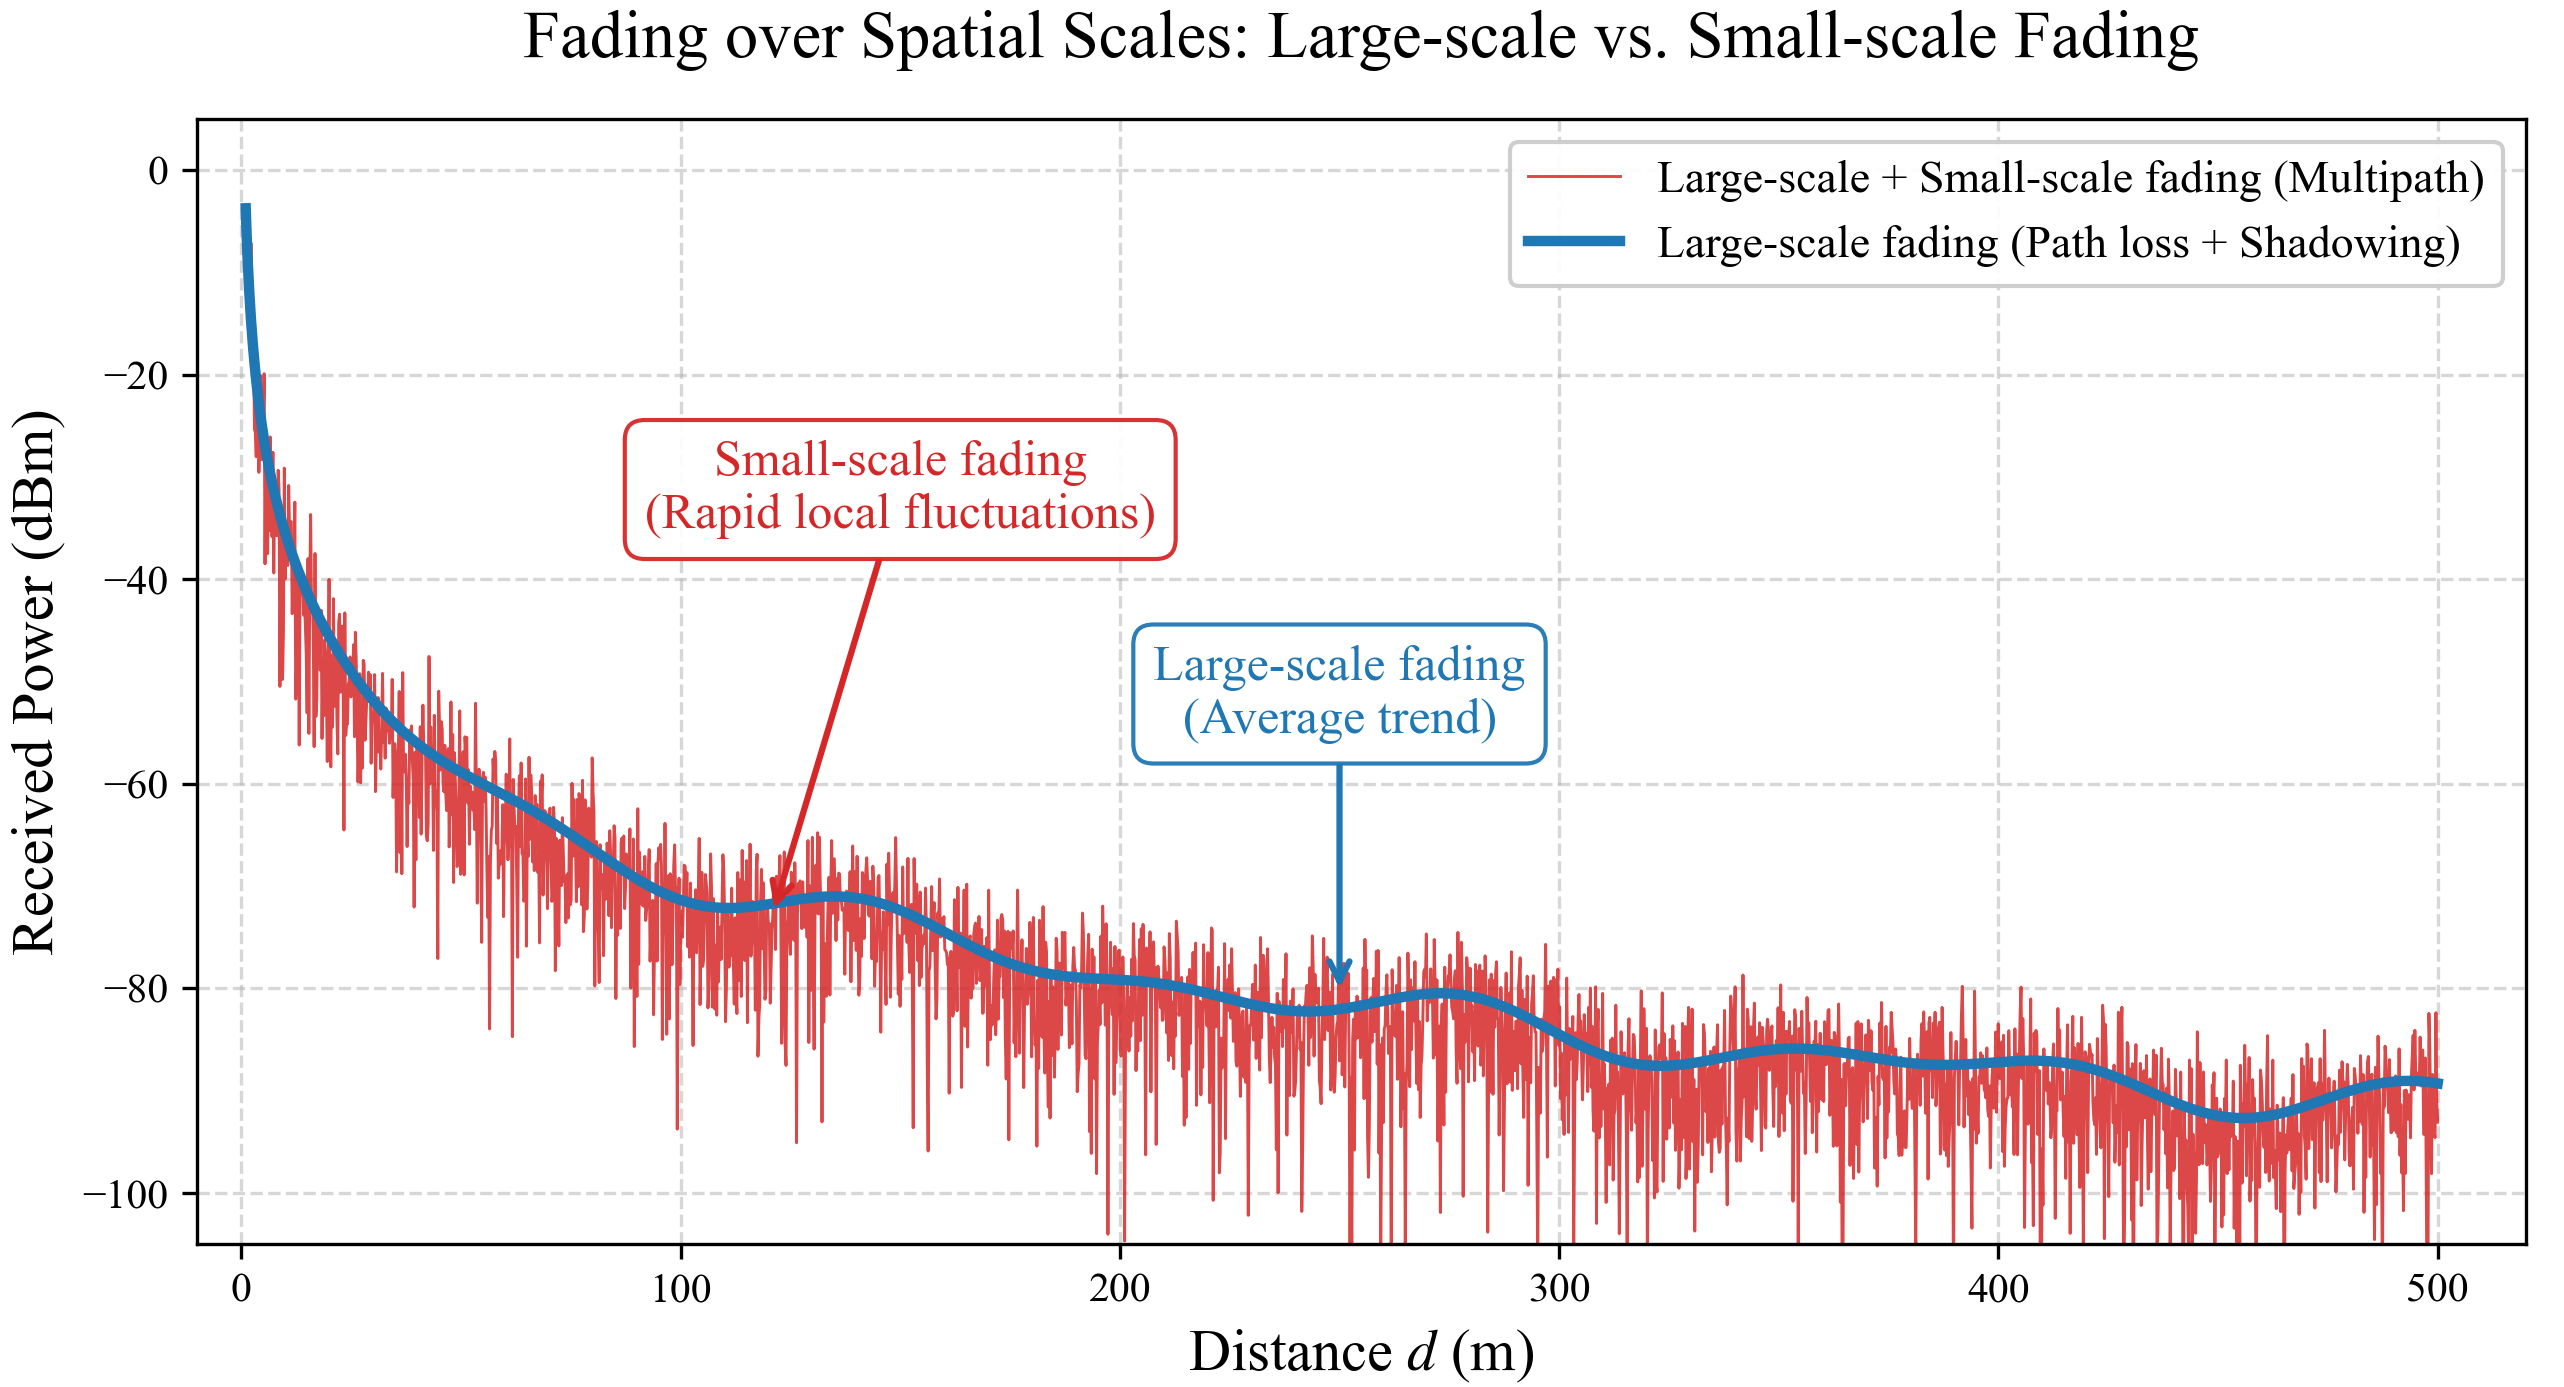
\includegraphics[width=0.66\textwidth]{figures/chapter2/fig_fading.png}
    \caption{Comparison between large-scale fading and small-scale fading.}
    \label{fig:spatial-fading}
\end{figure}
\noindent\textbullet\quad\textbf{From the time dimension: Doppler shift, coherence time, and fast/slow fading}

From the time dimension, fading is related to channel variation caused by
relative motion among the transmitter, receiver, or scatterers.
The resulting phase variation appears as a Doppler shift.
The maximum Doppler shift is usually written as
\begin{equation}
    f_D
    =
    \frac{v}{\lambda}
    =
    \frac{v f_c}{c},
    \label{eq:maximum-doppler-shift}
\end{equation}
where
\(v\) denotes the relative velocity,
\(\lambda\) denotes the carrier wavelength,
\(f_c\) denotes the carrier frequency,
and \(c\) denotes the speed of light.
Eq.~\eqref{eq:maximum-doppler-shift} shows that Doppler shift increases with
relative velocity and carrier frequency, making time variation more prominent
in high-mobility and high-frequency systems.

The \textbf{coherence time} \(T_c\) describes the time scale over which the
channel remains approximately unchanged and is roughly inversely proportional
to the maximum Doppler shift:
\begin{equation}
    T_c
    \propto
    \frac{1}{f_D}.
    \label{eq:coherence-time}
\end{equation}
A larger Doppler shift therefore implies a shorter coherence time and faster
channel variation.

Based on this concept,
the difference between slow fading and fast fading can be understood.
Let the symbol duration of the signal be \(T_s\).

\textbf{Slow fading} occurs when the channel varies slowly relative to the
signal.
If \(T_s \ll T_c\), the channel is nearly constant within one symbol duration.

\textbf{Fast fading} occurs when the channel varies rapidly relative to the
signal, for example when \(T_s\) is close to or larger than \(T_c\).
In this case, synchronization, channel estimation, and equalization become more
difficult.
Thus, slow and fast fading are determined by the relationship between the
channel-variation time scale and the signal time scale.

\noindent\textbullet\quad\textbf{From the frequency dimension: delay spread, coherence bandwidth, and frequency selectivity}

From the frequency dimension, fading is closely related to multipath delay
spread.
The root-mean-square delay spread \(\tau_{\mathrm{rms}}\) describes the
dispersion of multipath energy along the delay axis.
A larger delay spread usually leads to stronger variation of the channel
frequency response.

The \textbf{coherence bandwidth} \(B_c\) describes the frequency range over
which the channel response remains approximately consistent and is roughly
inversely proportional to the delay spread:
\begin{equation}
    B_c
    \propto
    \frac{1}{\tau_{\mathrm{rms}}}.
    \label{eq:coherence-bandwidth}
\end{equation}
A larger delay spread leads to a smaller coherence bandwidth.

\textbf{Flat fading} occurs when the signal bandwidth \(B\) is much smaller
than the coherence bandwidth \(B_c\), namely \(B \ll B_c\).
All frequency components then experience approximately the same channel
response, so the signal band can be represented by a single complex coefficient.

\textbf{Frequency-selective fading} occurs when \(B\) is close to or larger
than \(B_c\).
Different frequency components then experience different channel responses.
This is a central issue in wideband communication and motivates OFDM, which
divides a wideband signal into narrowband subcarriers that approximately
experience flat fading.

These fading types are not mutually exclusive; they describe wireless-channel
variation from spatial, temporal, and frequency perspectives.
For communication, fading is mainly an impairment to reliable transmission.
For ISAC, the quantities behind fading, such as delay, Doppler, angle, and path
gain, may also carry sensing information.
Table~\ref{tab:fading-types-comparison} summarizes the main sources, criteria,
and meanings of common fading types.
\begin{table}[htbp]
    \centering
    \caption{Comparison of different fading types.}
    \label{tab:fading-types-comparison}
    \small
    \renewcommand{\arraystretch}{1.25}
    \begin{tabularx}{\textwidth}{
        >{\raggedright\arraybackslash}p{0.14\textwidth}
        >{\raggedright\arraybackslash}p{0.19\textwidth}
        >{\raggedright\arraybackslash}p{0.22\textwidth}
        >{\centering\arraybackslash}p{0.14\textwidth}
        >{\raggedright\arraybackslash}X
    }
        \toprule
        \textbf{View}
        &
        \textbf{Type}
        &
        \textbf{Physical cause}
        &
        \textbf{Criterion}
        &
        \textbf{Key idea}
        \\
        \midrule

        Spatial scale
        &
        Large-scale fading
        &
        Path loss, shadowing, and blockage
        &
        Large-area power variation
        &
        Slow average-power change
        \\

        Spatial scale
        &
        Small-scale fading
        &
        Multipath superposition
        &
        Local power fluctuation
        &
        Rapid local fluctuation
        \\

        Time variation
        &
        Slow fading
        &
        Low mobility and small Doppler
        &
        \(T_s \ll T_c\)
        &
        Channel nearly constant within one symbol
        \\

        Time variation
        &
        Fast fading
        &
        High mobility or large Doppler
        &
        \(T_s \gtrsim T_c\)
        &
        Channel changes within one symbol
        \\

        Frequency response
        &
        Flat fading
        &
        Small delay spread
        &
        \(B \ll B_c\)
        &
        Similar response across bandwidth
        \\

        Frequency response
        &
        Frequency-selective fading
        &
        Large delay spread
        &
        \(B \gtrsim B_c\)
        &
        Different response across frequencies
        \\
        \bottomrule
    \end{tabularx}
\end{table}


\topichead{Communication Quality Metrics}

Path loss, multipath, fading, noise, and interference ultimately appear at the
receiver as changes in signal quality.
Communication systems therefore use layered performance metrics: link quality
metrics describe the received signal condition, reliability metrics describe
information recovery, and efficiency metrics describe resource utilization.

\textbf{Link quality metrics} include SNR and SINR.
The signal-to-noise ratio (SNR) is
\begin{equation}
    \mathrm{SNR}
    =
    \frac{P_s}{P_n},
    \label{eq:snr-definition}
\end{equation}
where
\(P_s\) denotes the useful signal power at the receiver,
and \(P_n\) denotes the noise power.
If the noise power spectral density is \(N_0\) and the bandwidth is \(B\),
\begin{equation}
    P_n
    =
    N_0 B.
    \label{eq:noise-power-bandwidth}
\end{equation}
When interference from other users, neighboring cells, or spectrum-sharing
devices is present, SINR is more suitable:
\begin{equation}
    \mathrm{SINR}
    =
    \frac{P_s}{P_i + P_n},
    \label{eq:sinr-definition}
\end{equation}
where
\(P_i\) denotes the interference power.
For ISAC, SINR is particularly important because communication signals, sensing
echoes, clutter, and multi-user interference may coexist over shared time,
frequency, spatial, and power resources.

\textbf{Reliability metrics} measure whether transmitted information is
correctly recovered.
The bit error rate (BER) is
\begin{equation}
    \mathrm{BER}
    =
    \frac{N_{\mathrm{error}}}{N_{\mathrm{total}}},
    \label{eq:ber-definition}
\end{equation}
where
\(N_{\mathrm{error}}\) denotes the number of bits incorrectly decided at the receiver,
and \(N_{\mathrm{total}}\) denotes the total number of transmitted bits.
A higher SNR or SINR generally reduces BER, whereas severe fading, stronger
interference, or higher noise increases it.
BER is also affected by modulation and channel coding: higher-order modulation
improves spectral efficiency but is more sensitive to noise, while coding
improves reliability at the cost of redundancy.
Block error rate (BLER) is often used in practical systems because it is
directly related to link adaptation, retransmission, and throughput.

\textbf{Efficiency metrics} describe how effectively limited time-frequency
resources are used.
For an ideal Gaussian channel, capacity provides an upper-bound reference:
\begin{equation}
    C
    =
    B \log_2
    \left(
        1+\mathrm{SNR}
    \right),
    \label{eq:capacity-snr}
\end{equation}
where
\(C\) denotes the channel capacity,
and \(B\) denotes the system bandwidth.
With interference treated as an additional noise-like term, SNR is often
replaced by SINR:
\begin{equation}
    C
    =
    B \log_2
    \left(
        1+\mathrm{SINR}
    \right).
    \label{eq:capacity-sinr}
\end{equation}
These formulas show that the rate reference depends on bandwidth and link
quality, but grows only logarithmically with SNR or SINR.
Throughput describes the amount of useful data successfully received per unit
time:
\begin{equation}
    R_{\mathrm{throughput}}
    =
    \frac{N_{\mathrm{success}}}{T},
    \label{eq:throughput-definition}
\end{equation}
where
\(N_{\mathrm{success}}\) denotes the number of information bits successfully received within time \(T\).
If \(R\) is the nominal transmission rate,
\begin{equation}
    R_{\mathrm{throughput}}
    \approx
    R
    \left(
        1-\mathrm{BLER}
    \right).
    \label{eq:throughput-bler}
\end{equation}
so a higher nominal rate does not necessarily imply higher useful throughput
when BLER is large.

Spectral efficiency measures the rate per unit bandwidth:
\begin{equation}
    \eta
    =
    \frac{R}{B},
    \label{eq:spectral-efficiency-definition}
\end{equation}
with the unit bit/s/Hz.
Using capacity as an ideal reference,
\begin{equation}
    \eta
    =
    \log_2
    \left(
        1+\mathrm{SNR}
    \right),
    \label{eq:spectral-efficiency-snr}
\end{equation}
or,
when interference is considered,
as
\begin{equation}
    \eta
    =
    \log_2
    \left(
        1+\mathrm{SINR}
    \right).
    \label{eq:spectral-efficiency-sinr}
\end{equation}
For ISAC, spectral efficiency is closely related to whether communication and
sensing can reuse spectrum, hardware, and waveform resources.
In summary, channel effects first influence SNR or SINR; SNR or SINR affects
BER and BLER; reliability then influences throughput; and under a given
bandwidth, the effective rate determines spectral efficiency.
These communication-side metrics provide the basis for later analysis of
communication--sensing tradeoffs, resource allocation, and joint optimization.

\topichead{Channel State Information}

To perform receiver processing and transmission optimization, a communication
system needs descriptive information about the current wireless channel, called
\textbf{channel state information} (CSI).
CSI captures amplitude attenuation, phase rotation, delay spread, frequency
selectivity, and spatial direction from the viewpoint of the communication
system.

The specific form of CSI depends on the system structure.
In a single-antenna narrowband system, CSI can be simplified as a complex
coefficient
\begin{equation}
    h
    =
    |h|e^{j\phi},
    \label{eq:csi-siso-coefficient}
\end{equation}
where
\(|h|\) describes the change in signal amplitude,
and \(\phi\) describes the change in signal phase.
In an OFDM system, CSI is represented by the frequency-domain channel response
on different subcarriers:
\begin{equation}
    H[k],
    \label{eq:csi-ofdm-subcarrier}
\end{equation}
where
\(k\) denotes the subcarrier index,
and \(H[k]\) describes the channel amplitude and phase variation on the \(k\)-th subcarrier.
In a MIMO system, CSI is represented as a channel matrix
\begin{equation}
    \mathbf{H},
    \label{eq:csi-mimo-matrix}
\end{equation}
whose elements describe the spatial relationships between transmit and receive
antennas.
Although CSI has different forms, its core role is always to describe how the
channel affects the transmitted signal.

CSI is usually estimated through pilot or reference signals known to the
receiver.
By comparing the transmitted pilots with the received pilot observations, the
receiver estimates the channel using methods such as LS, LMMSE, interpolation,
filtering, or compressed sensing, depending on system assumptions.
In OFDM and MIMO systems, this estimation is performed across subcarriers and
antenna pairs.

CSI acquisition also depends on the duplexing mode.
In FDD systems, downlink CSI usually needs to be fed back because uplink and
downlink use different frequency bands.
In TDD systems, channel reciprocity allows uplink pilots to support downlink
transmission design, although RF-chain calibration is often required in
practice.

CSI supports equalization, adaptive modulation and coding, power control, user
scheduling, resource allocation, retransmission design, and MIMO precoding.
In multi-user MIMO, it helps determine beamforming weights and select users for
spatial multiplexing on the same time-frequency resource.
Thus, CSI is a key foundation for adaptive transmission.

In ISAC, CSI has an additional sensing meaning.
Delay may correspond to range, Doppler may indicate target or scatterer motion,
angle may describe spatial direction, and path gain may reflect scattering
strength or material properties.
CSI therefore connects wireless propagation with both adaptive communication
and environmental sensing, and will reappear in OFDM channel estimation, MIMO
beamforming, and joint communication--sensing processing.


\subsection{MIMO and Beamforming Fundamentals}

Modern broadband wireless systems often combine OFDM with multi-antenna
processing.
As illustrated in Fig.~\ref{fig:mimo_ofdm_flow}, coded and modulated symbols
are assigned to subcarriers, organized into spatial data streams, and mapped to
transmit antennas through MIMO precoding.
After IFFT-based OFDM modulation and receiver FFT processing, each subcarrier
can be described by an equivalent MIMO input-output relationship.

\begin{figure}[htbp]
    \centering
    % Replace the following file with the final generated flowchart.
    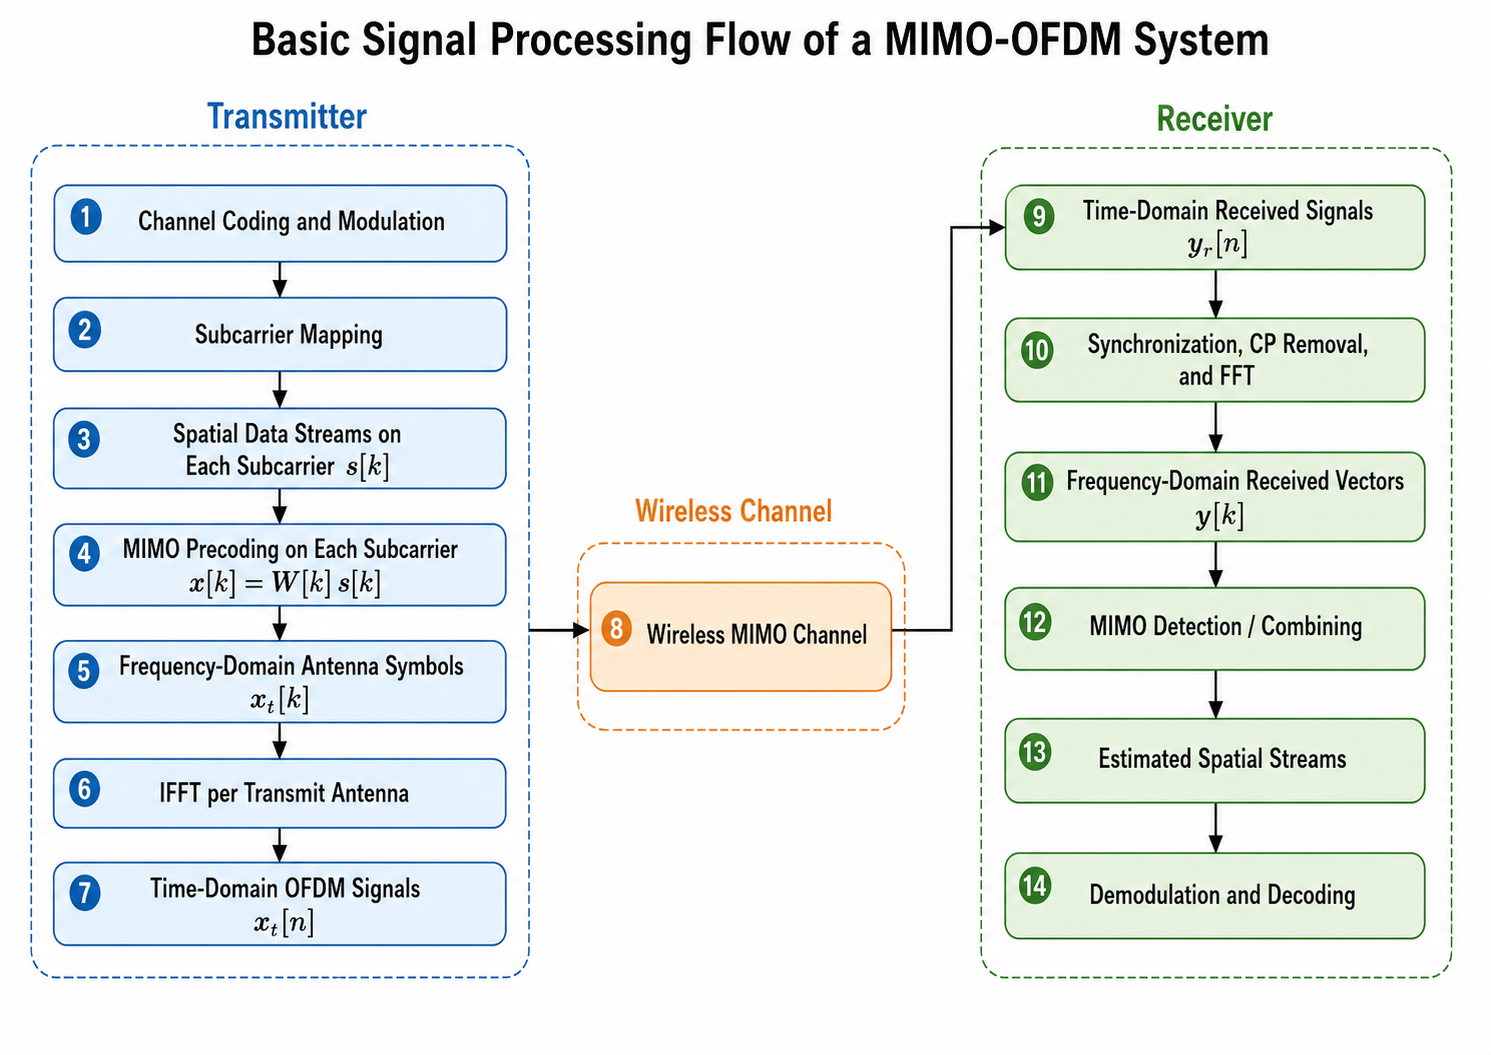
\includegraphics[width=0.72\textwidth]{figures/chapter2/fig_mimo_ofdm_flow.png}
    \caption{Basic signal processing flow of a MIMO-OFDM system.}
    \label{fig:mimo_ofdm_flow}
\end{figure}

In this subsection, \(\mathbf{x}[k]\) and \(\mathbf{y}[k]\) denote
frequency-domain antenna-symbol vectors on the \(k\)-th subcarrier, not the
complete time-domain OFDM waveform.
OFDM converts a wideband frequency-selective channel into narrowband subcarrier
channels, while MIMO exploits spatial degrees of freedom on each subcarrier.
\topichead{MIMO and the Spatial Dimension}
MIMO introduces the spatial dimension into the wireless link.
Compared with SISO, it turns the spatial domain into a design resource: the
system can transmit multiple streams on the same time-frequency resource,
improve reliability through multiple spatial paths, and enhance or suppress
signals through coherent antenna processing.
For ISAC, this spatial control is also the basis for target illumination, angle
estimation, and joint beam design.

\topichead{Basic MIMO Signal Model}
On the \(k\)-th subcarrier,
the equivalent input-output relationship of a MIMO system can be written as
\begin{equation}
\mathbf{y}[k]
=
\mathbf{H}[k]\mathbf{x}[k]
+
\mathbf{n}[k].
\label{eq:mimo_ofdm_subcarrier_model}
\end{equation}
Here, \(\mathbf{x}[k]\) and \(\mathbf{y}[k]\) are the transmit and receive
antenna-symbol vectors on the \(k\)-th subcarrier, \(\mathbf{n}[k]\) is the
noise vector, and \(\mathbf{H}[k]\) is the MIMO frequency-domain channel matrix.
This is an equivalent subcarrier-level model rather than a complete
time-domain OFDM waveform model.

If the transmitter and the receiver are equipped with \(N_t\) and \(N_r\) antennas, respectively,
then
\[
\mathbf{x}[k]\in\mathbb{C}^{N_t\times 1},
\quad
\mathbf{y}[k]\in\mathbb{C}^{N_r\times 1},
\quad
\mathbf{n}[k]\in\mathbb{C}^{N_r\times 1},
\quad
\mathbf{H}[k]\in\mathbb{C}^{N_r\times N_t}.
\]
The element \(h_{ij}[k]\) represents the channel from the \(j\)-th transmit
antenna to the \(i\)-th receive antenna.
Thus, \(\mathbf{H}[k]\) contains multiple spatial channel relationships and
provides the basis for spatial multiplexing, spatial diversity, array gain, and
beamforming.

\topichead{Beamforming and Spatial Processing}
Beamforming exploits the spatial structure of \(\mathbf{H}[k]\) by controlling
the amplitudes and phases across antennas.
With properly designed complex weights, the desired signal can be coherently
enhanced toward a user or direction, while leakage and interference can be
suppressed.
For ISAC, the same weights also affect target illumination and echo quality, so
beamforming is a basic tool for spatial energy control.

\topichead{Main Gains of MIMO}
Based on the MIMO channel representation, three fundamental gains are commonly
discussed: spatial multiplexing, spatial diversity, and array gain.
They correspond respectively to higher rate, improved reliability, and stronger
effective signal power.
Figure~\ref{fig:mimo_gains_comparison} provides a conceptual comparison of these three gains.

\begin{figure}[htbp]
    \centering
    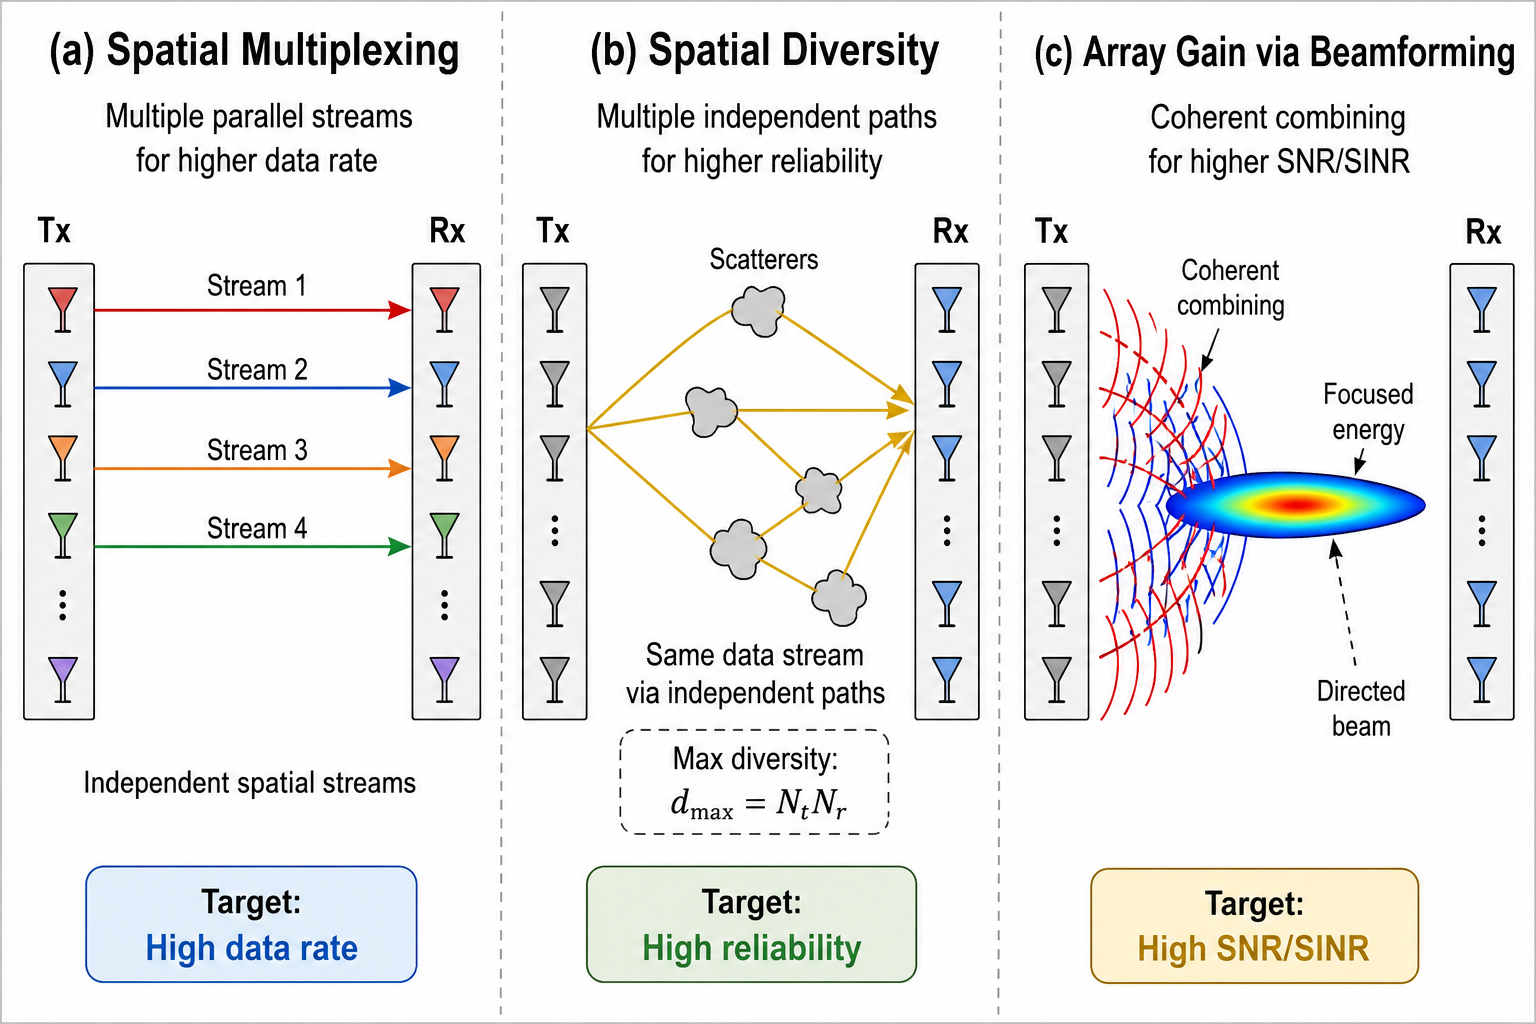
\includegraphics[width=0.72\textwidth]{figures/chapter2/fig_mimo_gain.png}
    \caption{Conceptual comparison of spatial multiplexing, spatial diversity, and array gain via beamforming in MIMO systems.}
    \label{fig:mimo_gains_comparison}
\end{figure}

As illustrated in Fig.~\ref{fig:mimo_gains_comparison}(a),
\textbf{spatial multiplexing} transmits multiple independent streams over the
same time-frequency resource through distinguishable spatial channels, thereby
improving throughput and spectral efficiency.
If the number of spatial streams transmitted on the \(k\)-th subcarrier is denoted by \(N_s\),
then the number of supportable spatial streams is usually limited by the rank of the channel matrix:
\begin{equation}
N_s
\leq
\operatorname{rank}\bigl(\mathbf{H}[k]\bigr)
\leq
\min(N_t,N_r).
\label{eq:mimo_spatial_stream_rank}
\end{equation}

As illustrated in Fig.~\ref{fig:mimo_gains_comparison}(b),
\textbf{spatial diversity} sends the same information through independent or
weakly correlated spatial paths, reducing the probability that all paths suffer
deep fading simultaneously.
Under ideal independent fading conditions,
if the system can fully exploit the spatial branches between \(N_t\) transmit antennas and \(N_r\) receive antennas,
the maximum spatial diversity order can be expressed as
\begin{equation}
d_{\max}
=
N_tN_r.
\label{eq:mimo_max_diversity_order}
\end{equation}
Here, \(d_{\max}\) denotes the maximum achievable diversity order.

\textbf{Array gain}, shown in Fig.~\ref{fig:mimo_gains_comparison}(c),
enhances the desired signal through coherent transmission or combining across
antennas, increasing the effective SNR or SINR.

In practical systems, these gains may appear together, but their design
objectives differ: rate, reliability, and signal strength.
Beamforming is one important method for realizing array gain, interference
suppression, and spatial selectivity.

\topichead{Transmit Precoding and Receive Processing}
MIMO gains require spatial processing at the transmitter and receiver.
On the \(k\)-th subcarrier, the transmitter maps the spatial data-stream vector
onto antenna ports:
\begin{equation}
\mathbf{x}[k]
=
\mathbf{W}[k]\mathbf{s}[k].
\label{eq:mimo_precoding}
\end{equation}
The dimensions of the related quantities are
\[
\mathbf{s}[k]\in\mathbb{C}^{N_s\times 1},
\quad
\mathbf{W}[k]\in\mathbb{C}^{N_t\times N_s},
\quad
\mathbf{x}[k]\in\mathbb{C}^{N_t\times 1}.
\]
Here, \(\mathbf{s}[k]\) is the spatial data-stream vector, \(N_s\) is the
number of streams, and \(\mathbf{W}[k]\) is the transmit precoding matrix that
maps streams to antenna-port symbols with selected amplitudes and phases.

Substituting the precoded transmit vector into the MIMO subcarrier model gives
\begin{equation}
\mathbf{y}[k]
=
\mathbf{H}[k]\mathbf{W}[k]\mathbf{s}[k]
+
\mathbf{n}[k].
\label{eq:mimo_precoded_channel}
\end{equation}
The product \(\mathbf{H}[k]\mathbf{W}[k]\) is the effective channel after
precoding, and \(\mathbf{y}[k]\) is generally a mixture of spatial streams.

The receiver then applies combining or detection.
Let \(\mathbf{G}[k]\in\mathbb{C}^{N_s\times N_r}\) denote the receive
processing matrix:
\[
\hat{\mathbf{s}}[k]
=
\mathbf{G}[k]\mathbf{y}[k],
\]
where
\(\hat{\mathbf{s}}[k]\in\mathbb{C}^{N_s\times 1}\)
is the estimate of the spatial data-stream vector.
By substituting \(\mathbf{y}[k]\) into the above expression,
the overall equivalent input-output relationship becomes
\begin{equation}
\hat{\mathbf{s}}[k]
=
\mathbf{G}[k]\mathbf{H}[k]\mathbf{W}[k]\mathbf{s}[k]
+
\mathbf{G}[k]\mathbf{n}[k].
\label{eq:mimo_end_to_end_model}
\end{equation}
The end-to-end MIMO process is therefore composed of transmit precoding,
wireless propagation, and receive processing.

Spatial multiplexing often uses detectors such as \acs{ZF} or MMSE to separate
streams; spatial diversity uses combining or space-time coding; and array gain
uses coherent transmission or combining.
MIMO gains therefore arise from the joint effect of precoding, propagation, and
receive processing, not merely from adding antennas.

\topichead{Connection to ISAC}
From the communication perspective, MIMO and beamforming improve rate,
reliability, effective received signal strength, and interference suppression.
From the sensing perspective, they control spatial illumination and obtain
direction information from array observations.
In ISAC, the same spectrum, hardware, waveform, and antenna array may serve
both users and sensing targets, so beam design must balance communication rate,
interference suppression, target echo strength, and angle estimation.
The spatial-channel, precoding, and receive-processing concepts introduced here
therefore form a key foundation for MIMO-ISAC and spatial resource allocation.


